When a $W$ boson decays to a neutrino and a lepton (including hadronically decaying $\tau$ and light leptons), the presence of neutrinos
in the final state results in \MET. The event passes the electron and muon veto because either the hadronically decaying $\tau$ is reconstructed
as a jet or the light leptons get ``lost" (from three reasons as described in the introduction). Although an isolated track veto is applied,
there are residual events passing because of the veto in-efficiency.
This background is estimated using control region of single lepton events selected from data using search trigger. Both muon and electron
control sample (CS) are used to improve the statistical uncertainty. Muon CS consists of $\mu$\,+\,jets events selected requiring exactly one
$\mu$ with $p_{T}^{\mu}>10 GeV$ and $|\eta|<2.4$. Similarly electron CS event is required to have exactly one electron with $p_{T}^{e}>10 GeV$ and $|\eta|<2.5$.
A cut on the transverse mass of the $W$, $m_\mathrm{T}=\sqrt{2p_{T}^{l}\MET(1-\cos\Delta\phi)}<$ 100 GeV, is required in order to select events
containing a $W\to$l$\nu$ decay and to suppress possible new physics signal contamination, i.e., signal events present in the $l$\,+\,jets sample.
Here, $l$ indicates both electron and $\mu$ and $\Delta\phi$ is the azimuthal angle between the $\vec{p_{T}}^l$ and the $\vec{\MET}$ directions.

In order to predict the number of events in signal regions, we measure so called ``translation factor" (TF) from simulation which is defined as $TF^{i} = N_{SR}^{i}/N_{CS}^{i}$,
where $N_{SR}^{i}$ is the number of either hadronic tau or lost lepton events in the $i^{th}$ signal region and $N_{CS}^{i}$ is the number of CS events in the corresponding signal region.
Apart from the difference of the $W$ boson decay, the CS and signal region have similar hadronic activities. However the complication comes from that \tauh is reconstructed as a jet
and addtional neutrino comes out of the \tauh decay in the hadronically decaying $\tauh$ case.

Generally our simulation of the \ttbar , $W$+jets and single-top have good agreement with data. However some differences are observed. In order to make simulation agree better
with data, we apply various officially provided data/MC scale factors. Since the translation factor takes a ratio of events between signal region and CS in the same simulated samples,
some data/MC scale factor effects cancel and have reduced effect on the measured factors. More details on TF are described in the section~\ref{sec:hadtauTF}. Two different
translation facotrs are obtained from $\mu$ and $e$ CS separately. By applying these factors to the corresponding data CS, hadronic tau or lost lepton events are estimated in search region
(Sec.~\ref{sec:hadtauprediction}). Systematic uncertainties on this method are addressed in Sec.~\ref{sec:hadtausys}.

A single translation factor in each search region is evaluated from simulated \ttbar, $W$+jets, and single-top events. The ratio of \tauh or lost lepton events after full search selection cuts to the lepton CS events selected with criteria discussed in Sec.~\ref{sec:hadtauCS} determines the translation factor. Two sets of TF are measured for $\mu$ and $e$ CS separately. To account for the difference in kinematic modeling between data and MC, three scale factors as mentioned in Sec.~\ref{sec:hadtauCS} are applied both on \tauh and CS events. The uncertainty on these scale factors are considered as systematic uncertainty,
all the possible source of data and MC differences are considered in systematic uncertainty evaluation (Sec.~\ref{sec:hadtausys}). %The b-tag SF and ISR re-weighting can be applied easily on the CS and \tauh events because of the presence of jets in both cases. But the way of applying lepton efficiency SF on \tauh is not straigh forward as there is no reconstructed and isolated lepton in \tauh after lepton veto.

The data-corrected translation facotrs for lepton control sample are shown in figure~\ref{fig:hadtau_TF} for the \tauh and figure~\ref{fig:lostle_TF} for the lost lepton for both muon and electron CS. As we expect, within uncertainties the TF from electron and muon CS follow similar trend across all the search bins.

\begin{figure}[htbp]
  \begin{center}
  \begin{tabular}{c}
  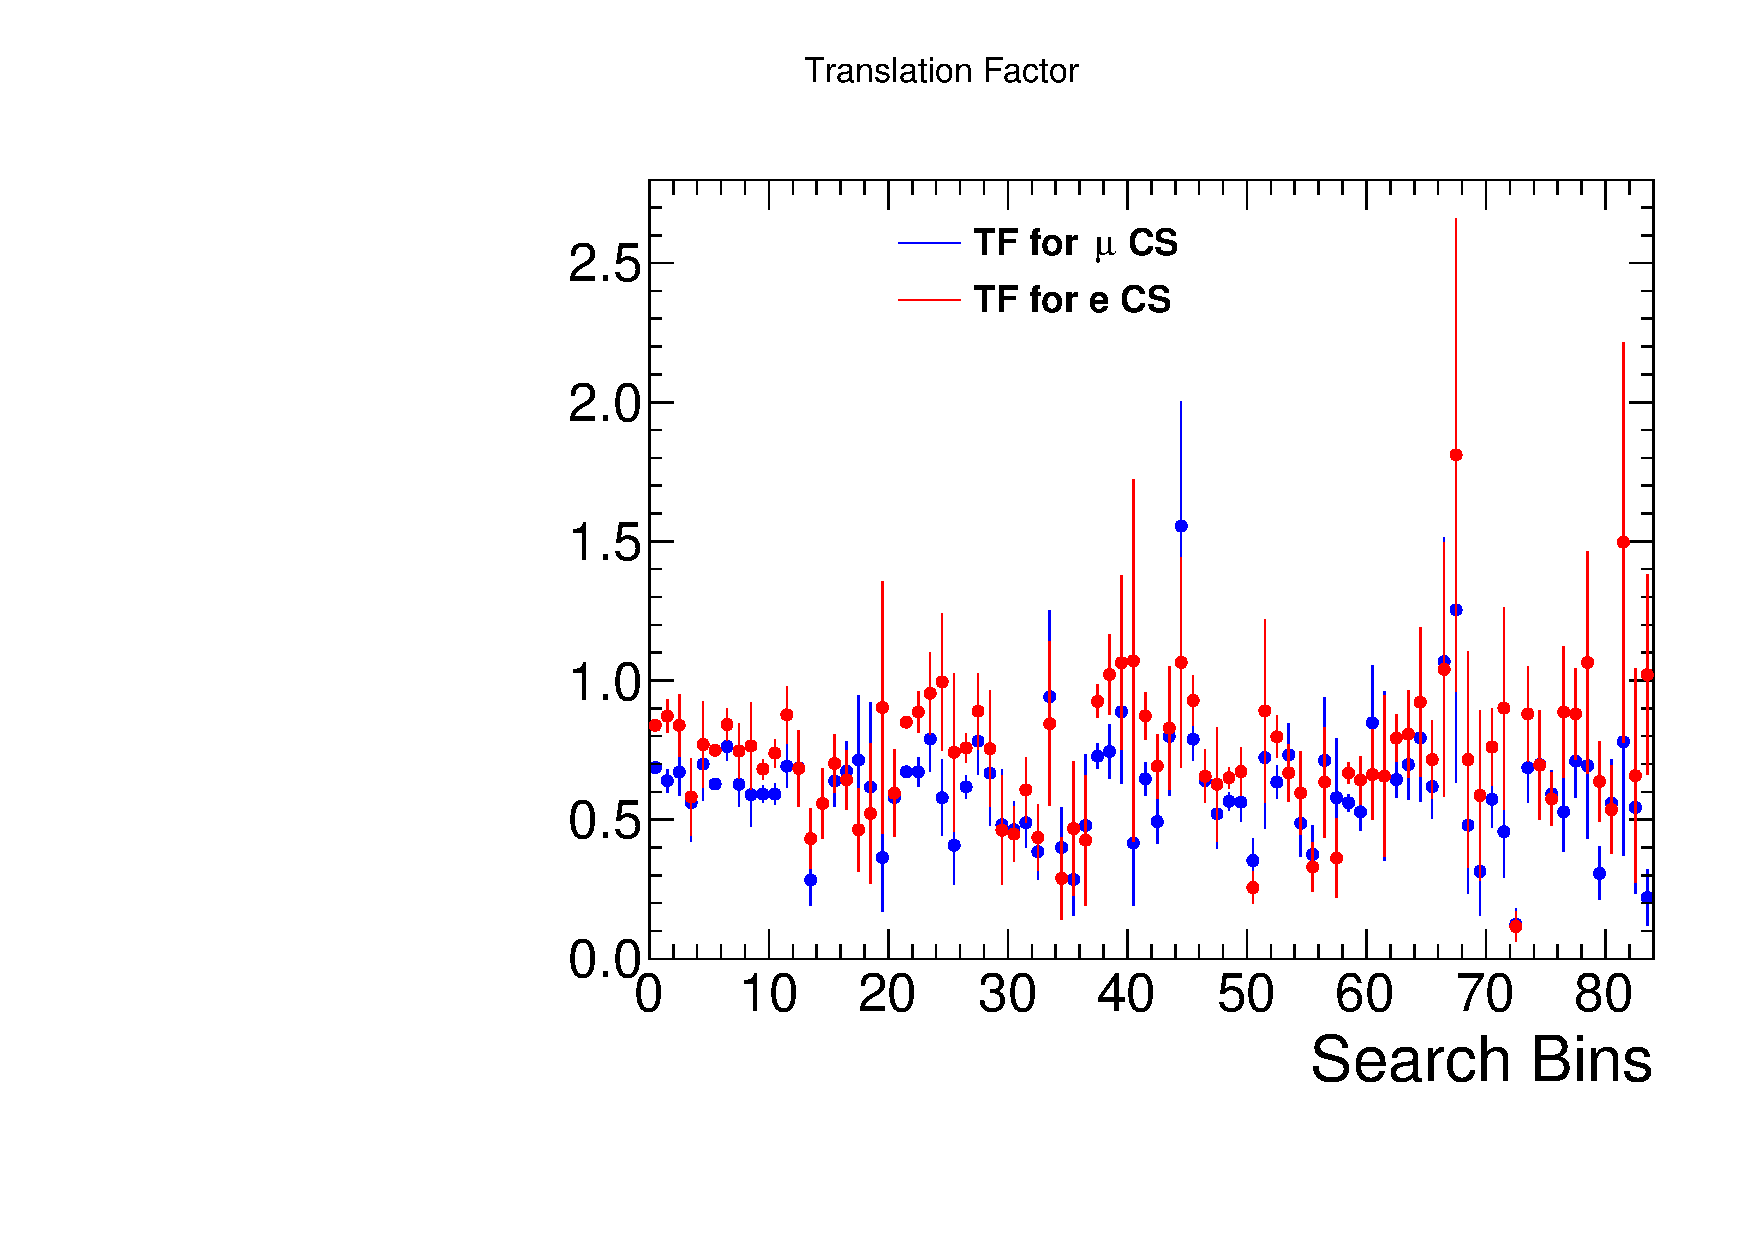
\includegraphics[angle=0,width=0.60\textwidth]{sections/mc4/Backgrounds/TF/figures/comp_TF_hadtau_comb.pdf}
  \end{tabular}
  \caption{Translation factors for the \tauh background prediction with their uncentainties from limited MC statistics for both muon and electron CS}
    \label{fig:hadtau_TF}
  \end{center}
\end{figure}


\begin{figure}[htbp]
  \begin{center}
  \begin{tabular}{c}
  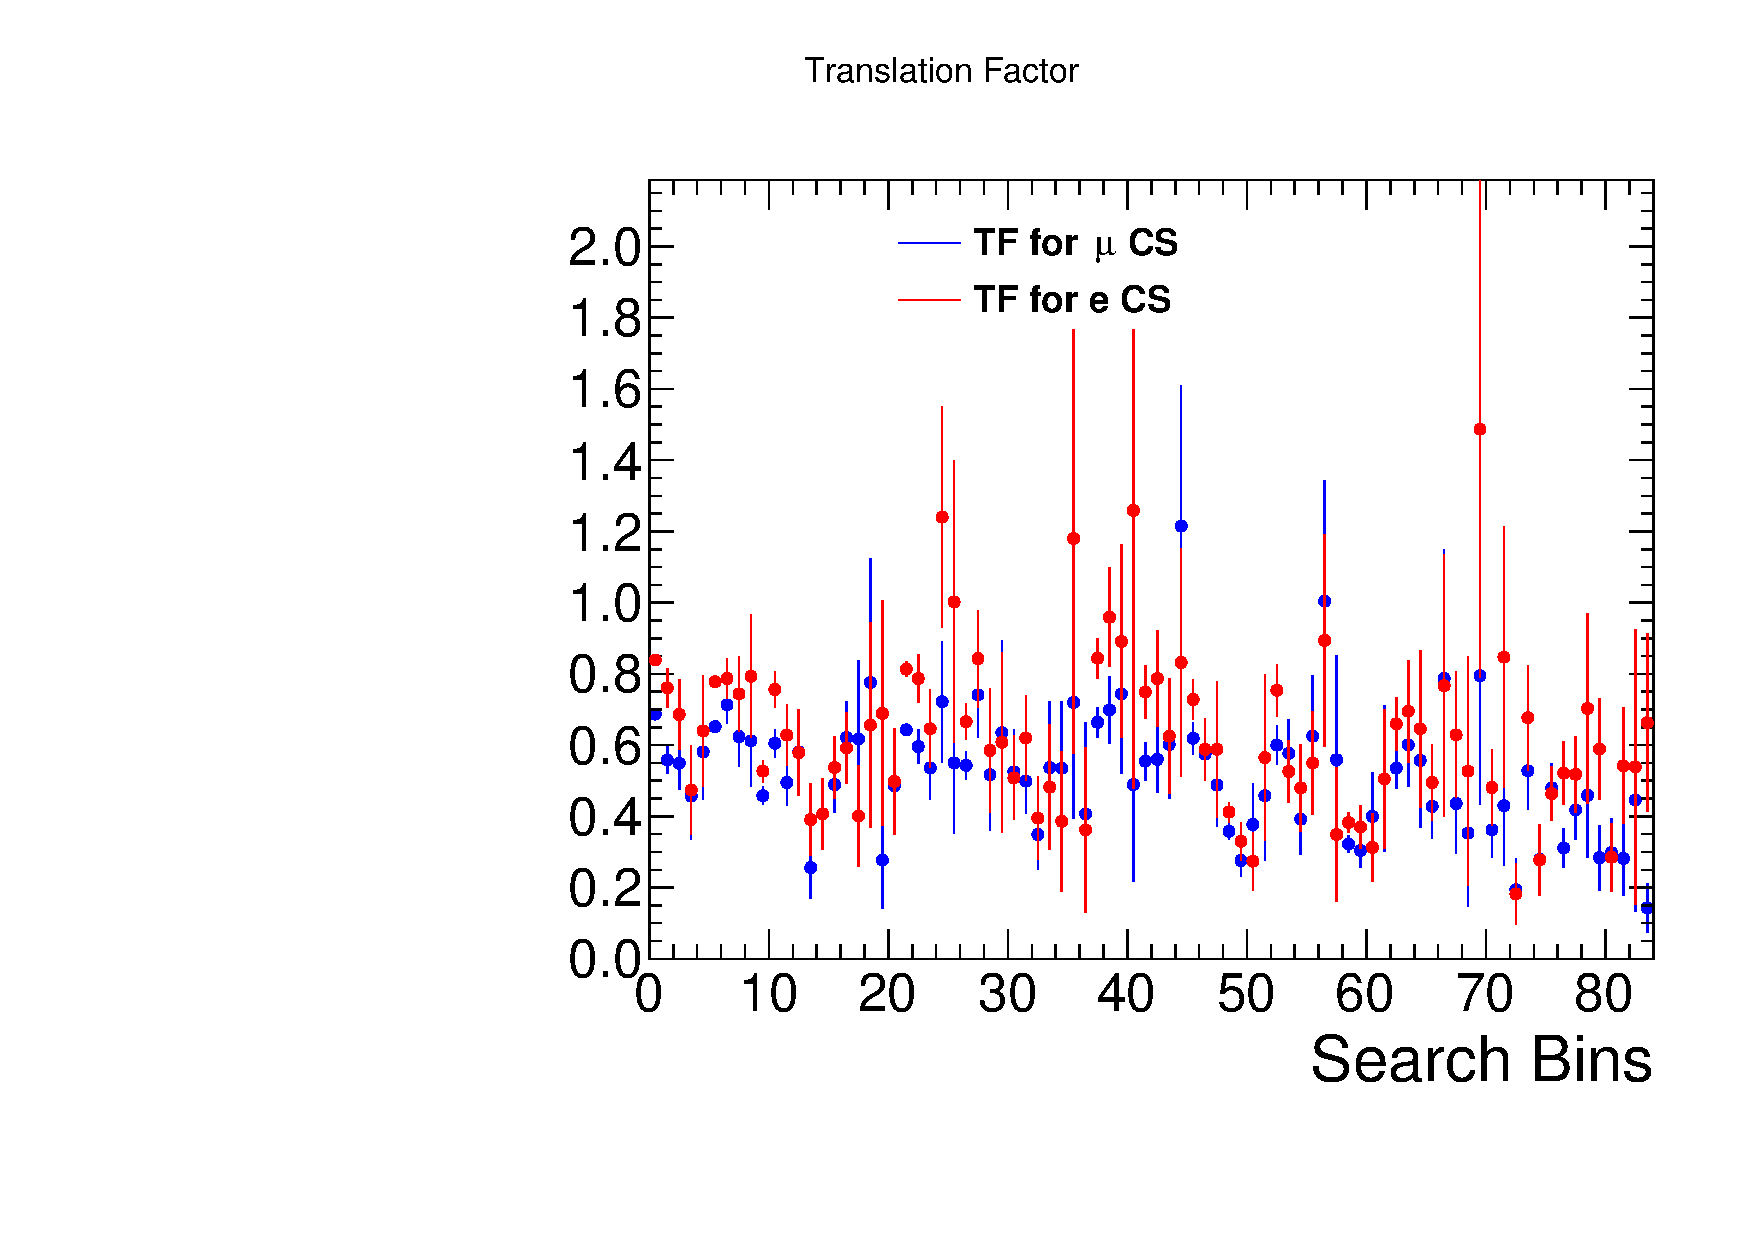
\includegraphics[angle=0,width=0.60\textwidth]{sections/mc4/Backgrounds/TF/figures/comp_TF_lostle_comb.pdf}
  \end{tabular}
  \caption{Translation factors for the lost lepton background prediction with their uncentainties from limited MC statistics for both muon and electron CS}
    \label{fig:lostle_TF}
  \end{center}
\end{figure}

In order to validate the method, we need a data sideband (0t2b) enriched with \ttbar, $W$+jets and single-top events. Therefore we select an orthogonal sideband w.r.t. signal region by inverting \ntops requirement, i.e., $\ntops=0$. In this region, we have significant amount of contributions from QCD and $Z \rightarrow \nu \nu$ processes. Therefore we apply additional $\nbjets\geq2$ and tighter $\Delta\phi(\MET, j_{1,2,3,4})>$ 0.5 cuts to further reduce QCD and $Z \rightarrow \nu \nu$ backgrounds. In this sideband, we use the same TF method to make the \ttbar, $W$+jets and signle-top background predictions. For other background components, MC yields are directly used. Specifically for the $Z \rightarrow \nu \nu$, we check that the scale is approximately 1.0 from MC yields to the data-driven result. In figure~\ref{fig:val_0t2b_mu} and figure~\ref{fig:val_0t2b_el}, we have the observed data yields compared to total backgrounds where the TF method is used for \ttbar, $W$+jets and single-top prediction. They clearly show that for both muon and electron channels, our TF methods work well to make the predictions in the sideband.

\begin{figure}[htbp]
  \begin{center}
  \begin{tabular}{c}
  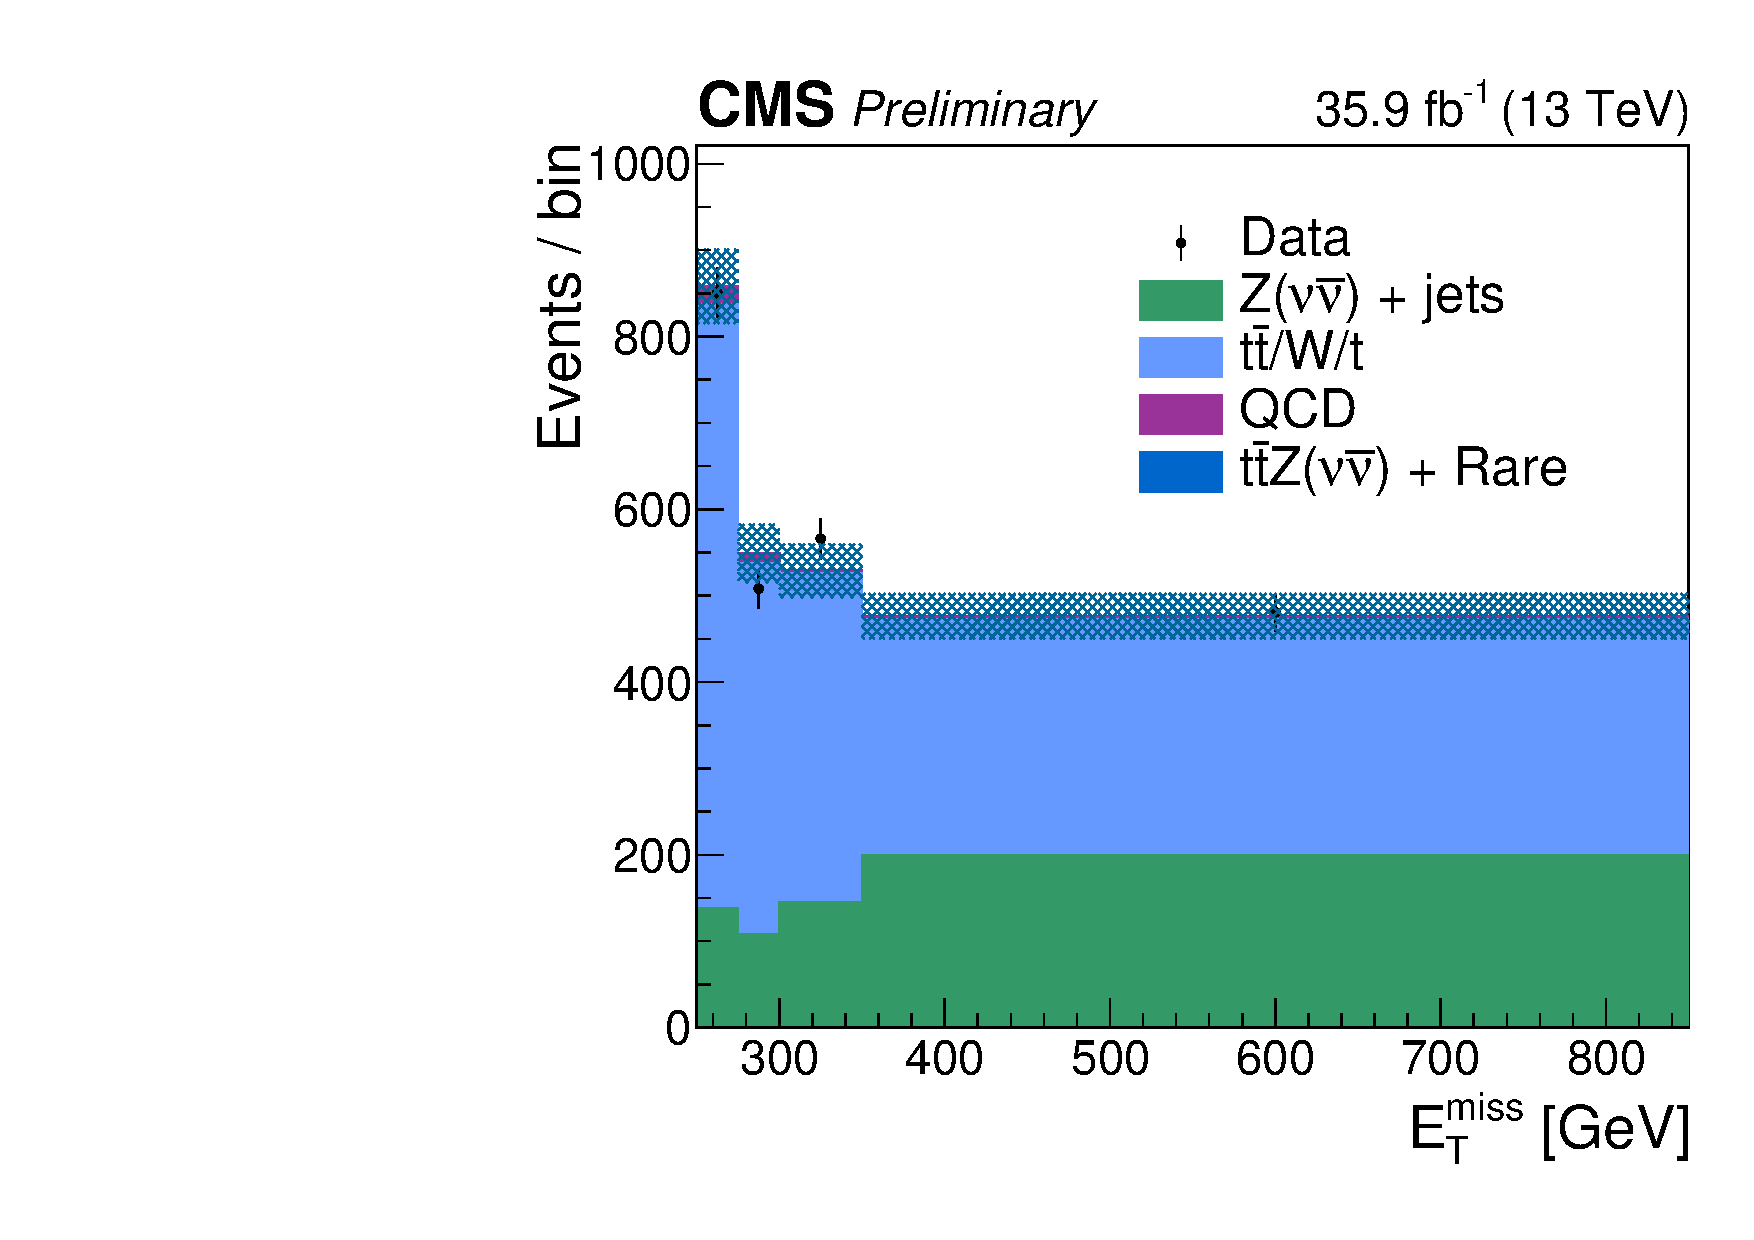
\includegraphics[angle=0,width=0.75\textwidth]{sections/mc4/Backgrounds/TF/figures/stack_2b0t_mu.pdf}
  \end{tabular}
  \caption{Validation of TF method in the 0t2b sideband from the muon channel. The black points are observed data. The light blue is predicted \ttbar, $W$+jets and single-top events using TF method. All other backgrounds directly come from MC yields. The errors include only statistcal uncertainties.}
    \label{fig:val_0t2b_mu}
  \end{center}
\end{figure}

\begin{figure}[htbp]
  \begin{center}
  \begin{tabular}{c}
  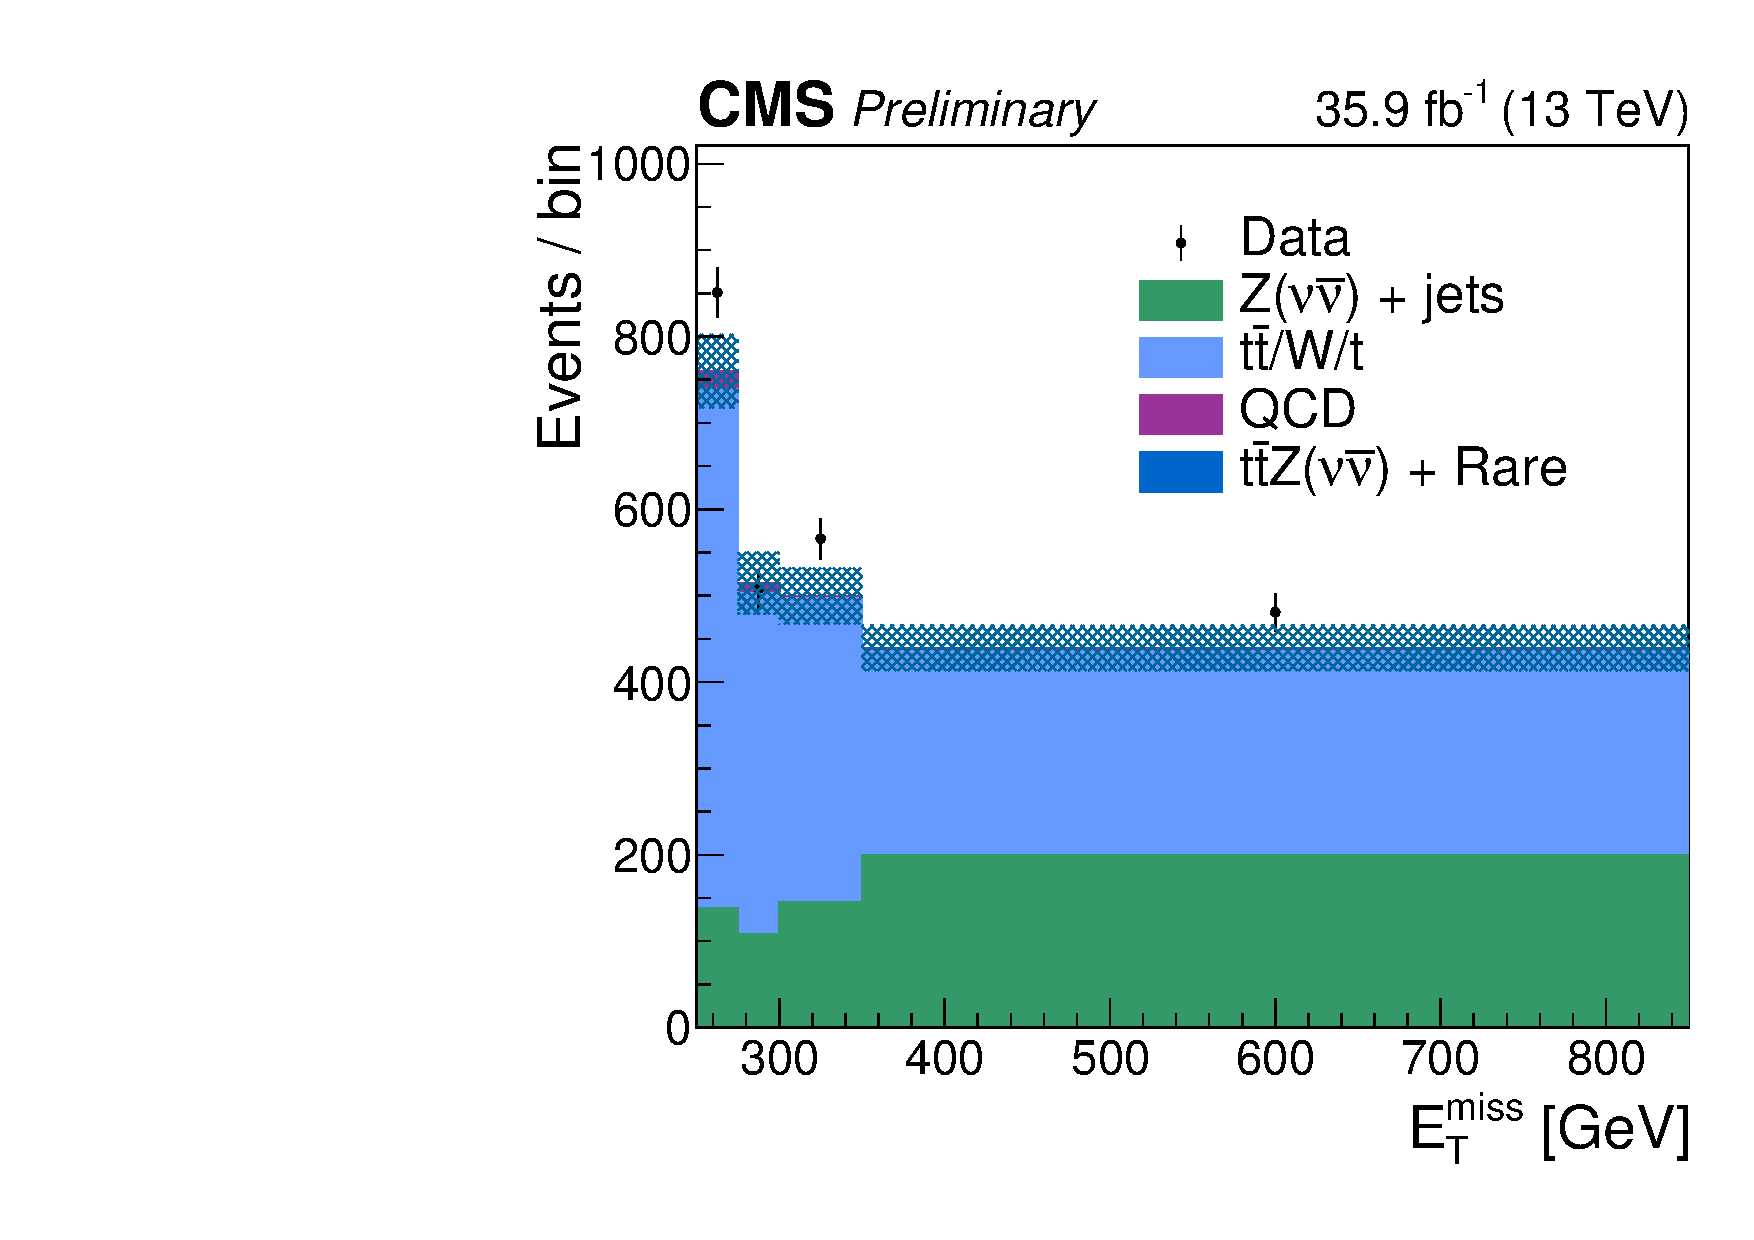
\includegraphics[angle=0,width=0.75\textwidth]{sections/mc4/Backgrounds/TF/figures/stack_2b0t_el.pdf}
  \end{tabular}
  \caption{Validation of TF method in the 0t2b sideband from the electron channel. The black points are observed data. The light blue is predicted \ttbar, $W$+jets and single-top events using TF method. All other backgrounds directly come from MC yields. The errors include only statistcal uncertainties.}
    \label{fig:val_0t2b_el}
  \end{center}
\end{figure}

After applying the measured TF from simulation on data CS events we can obtain the hadronic tau background predictions.
Since we have data CS from both electron and muon channels, we avarge predictions from both CS to make the final numbers.
Fig~\ref{fig:TAUpredictionSB} and fig~\ref{fig:LLpredictionSB} show the predictions for all search regions. The error bars in the figures
include both statistic and total systematic uncertainties. The statistical uncertainties are propagation of the Poisson statistics of the observed data CS events from both electron and                                                                             
muon channels given by the Garwood interval~\cite{GarwoodIntervalTwiki}.
In the statistical interpretation of the search discussed in section~\ref{sec:interpretation}, this Poisson uncertainty
is treated in the Higgs combination tool using a gamma function~\cite{HiggsCombine,cms-note-2011-005}.

\begin{figure}[htbp]
  \begin{center}
  \begin{tabular}{cc}
  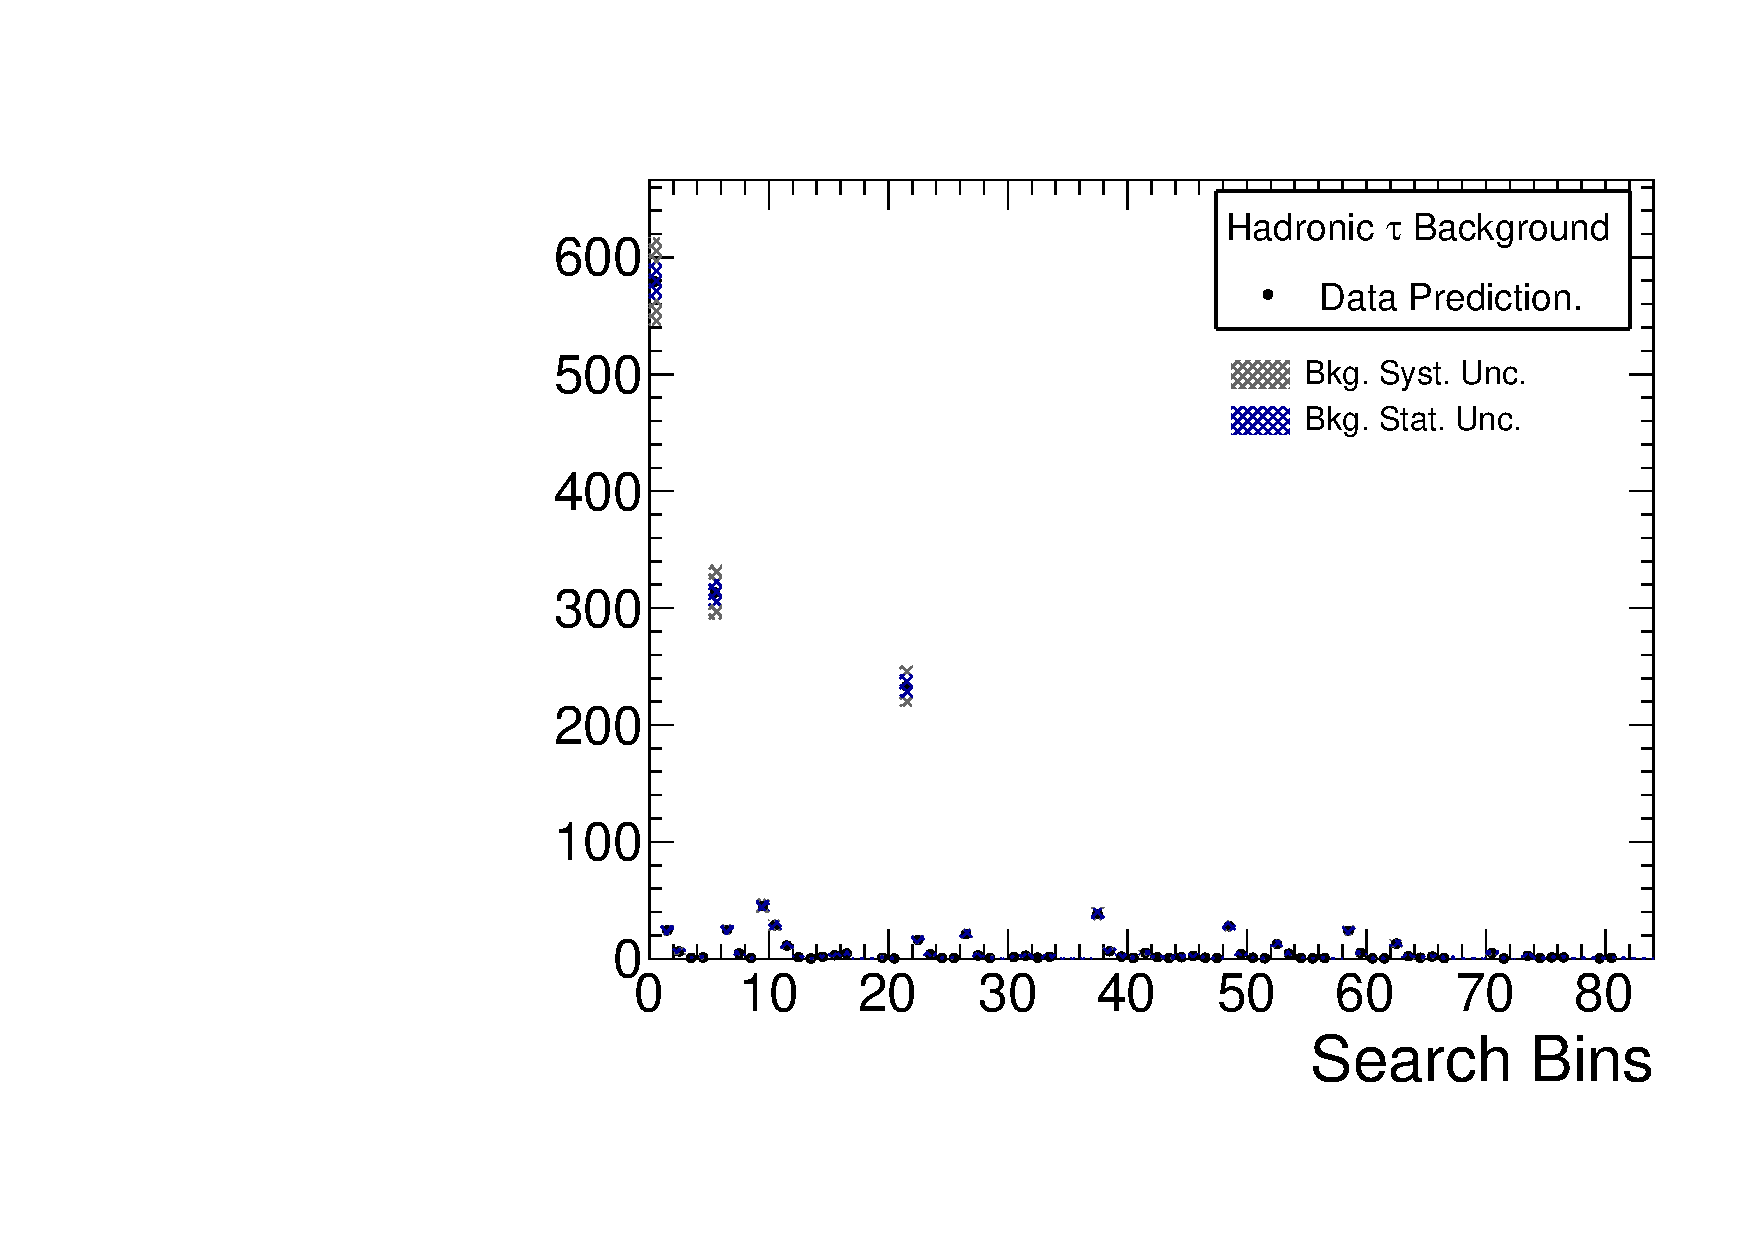
\includegraphics[angle=0,width=0.5\textwidth]{sections/mc4/Backgrounds/TF/figures/pred_full_hadtau_comb.pdf}
  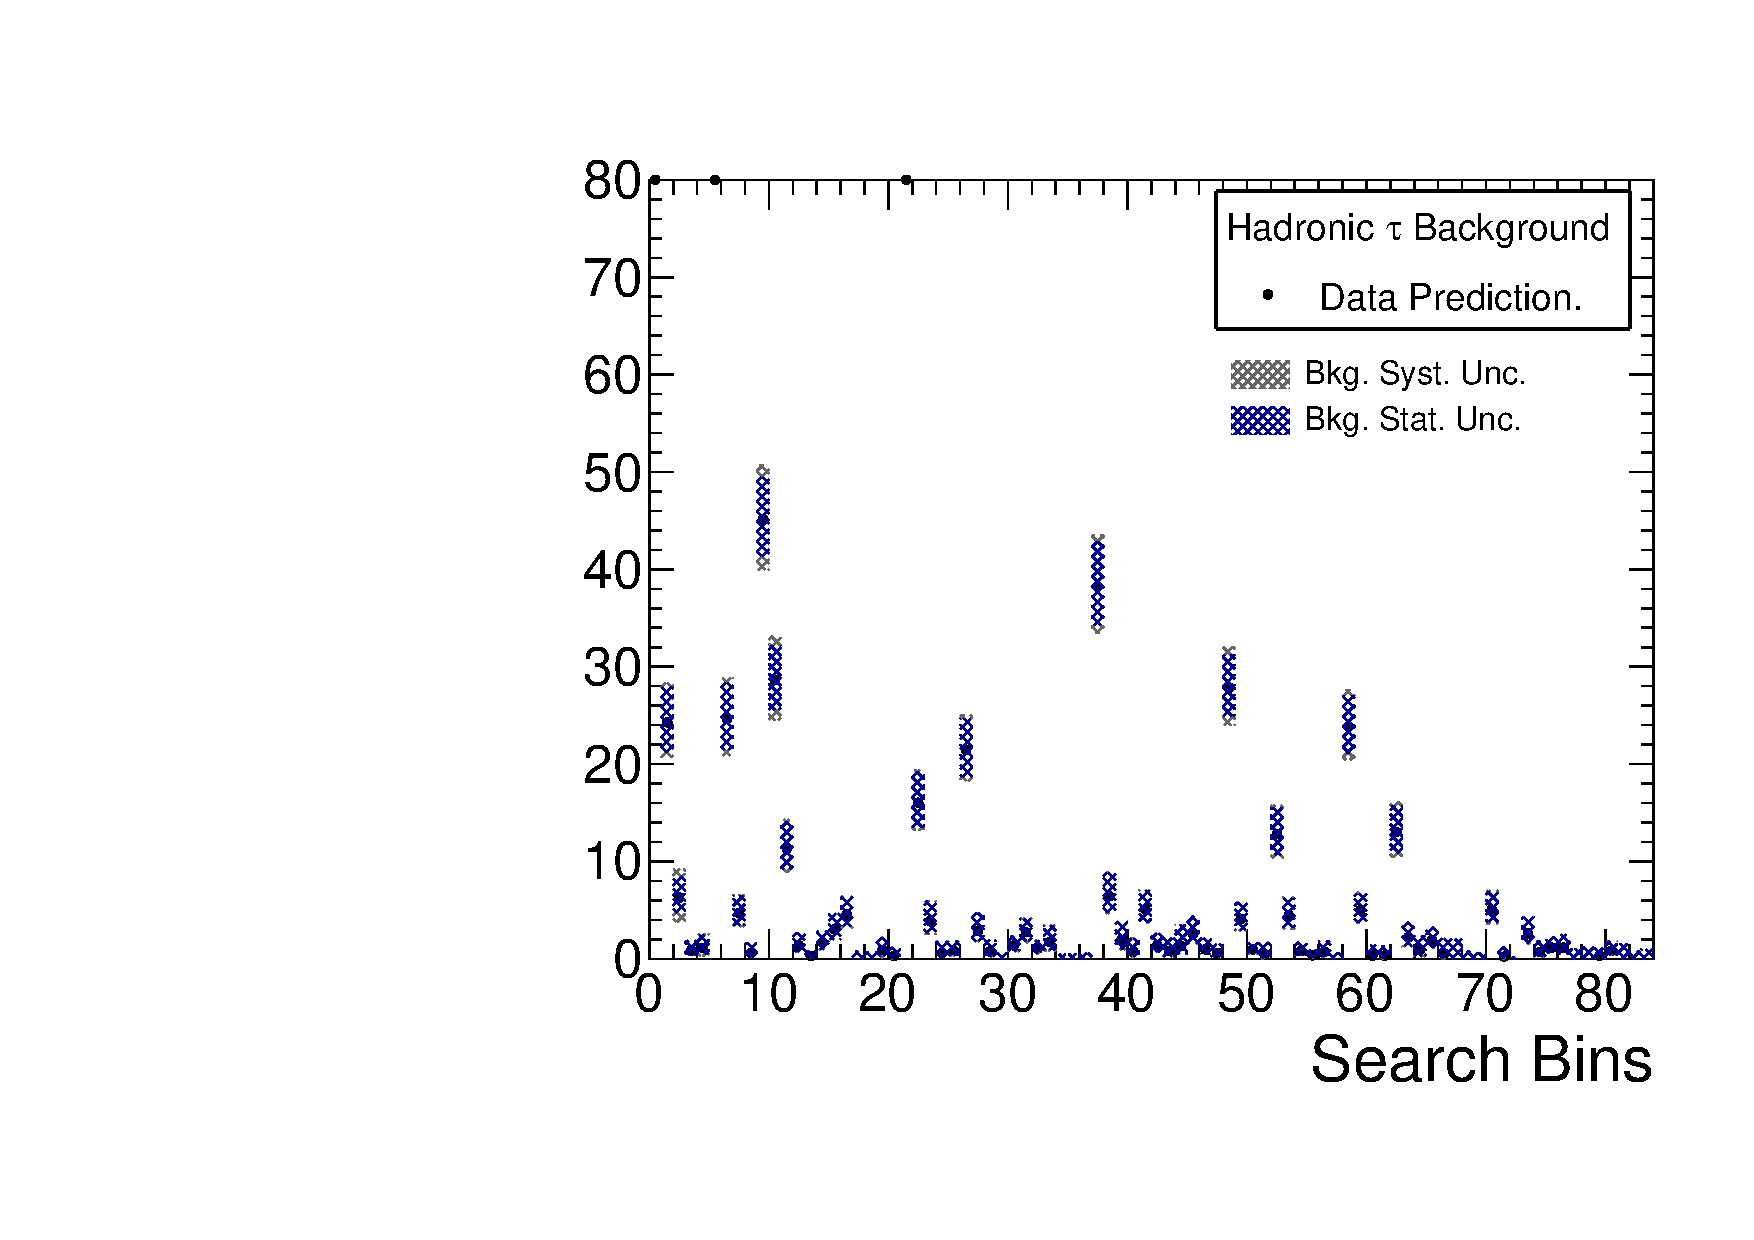
\includegraphics[angle=0,width=0.5\textwidth]{sections/mc4/Backgrounds/TF/figures/pred_zoomin_hadtau_comb.pdf}
  \end{tabular}
  \caption{Predicted hadronic tau background yield for a $35.9$~fb$^{-1}$ data for all the search regions. Right plot is a zoomed version of left plot.
Both statistical and total systematic uncertainties are shown. }
    \label{fig:TAUpredictionSB}
  \end{center}
\end{figure}

\begin{figure}[htbp]
  \begin{center}
  \begin{tabular}{cc}
  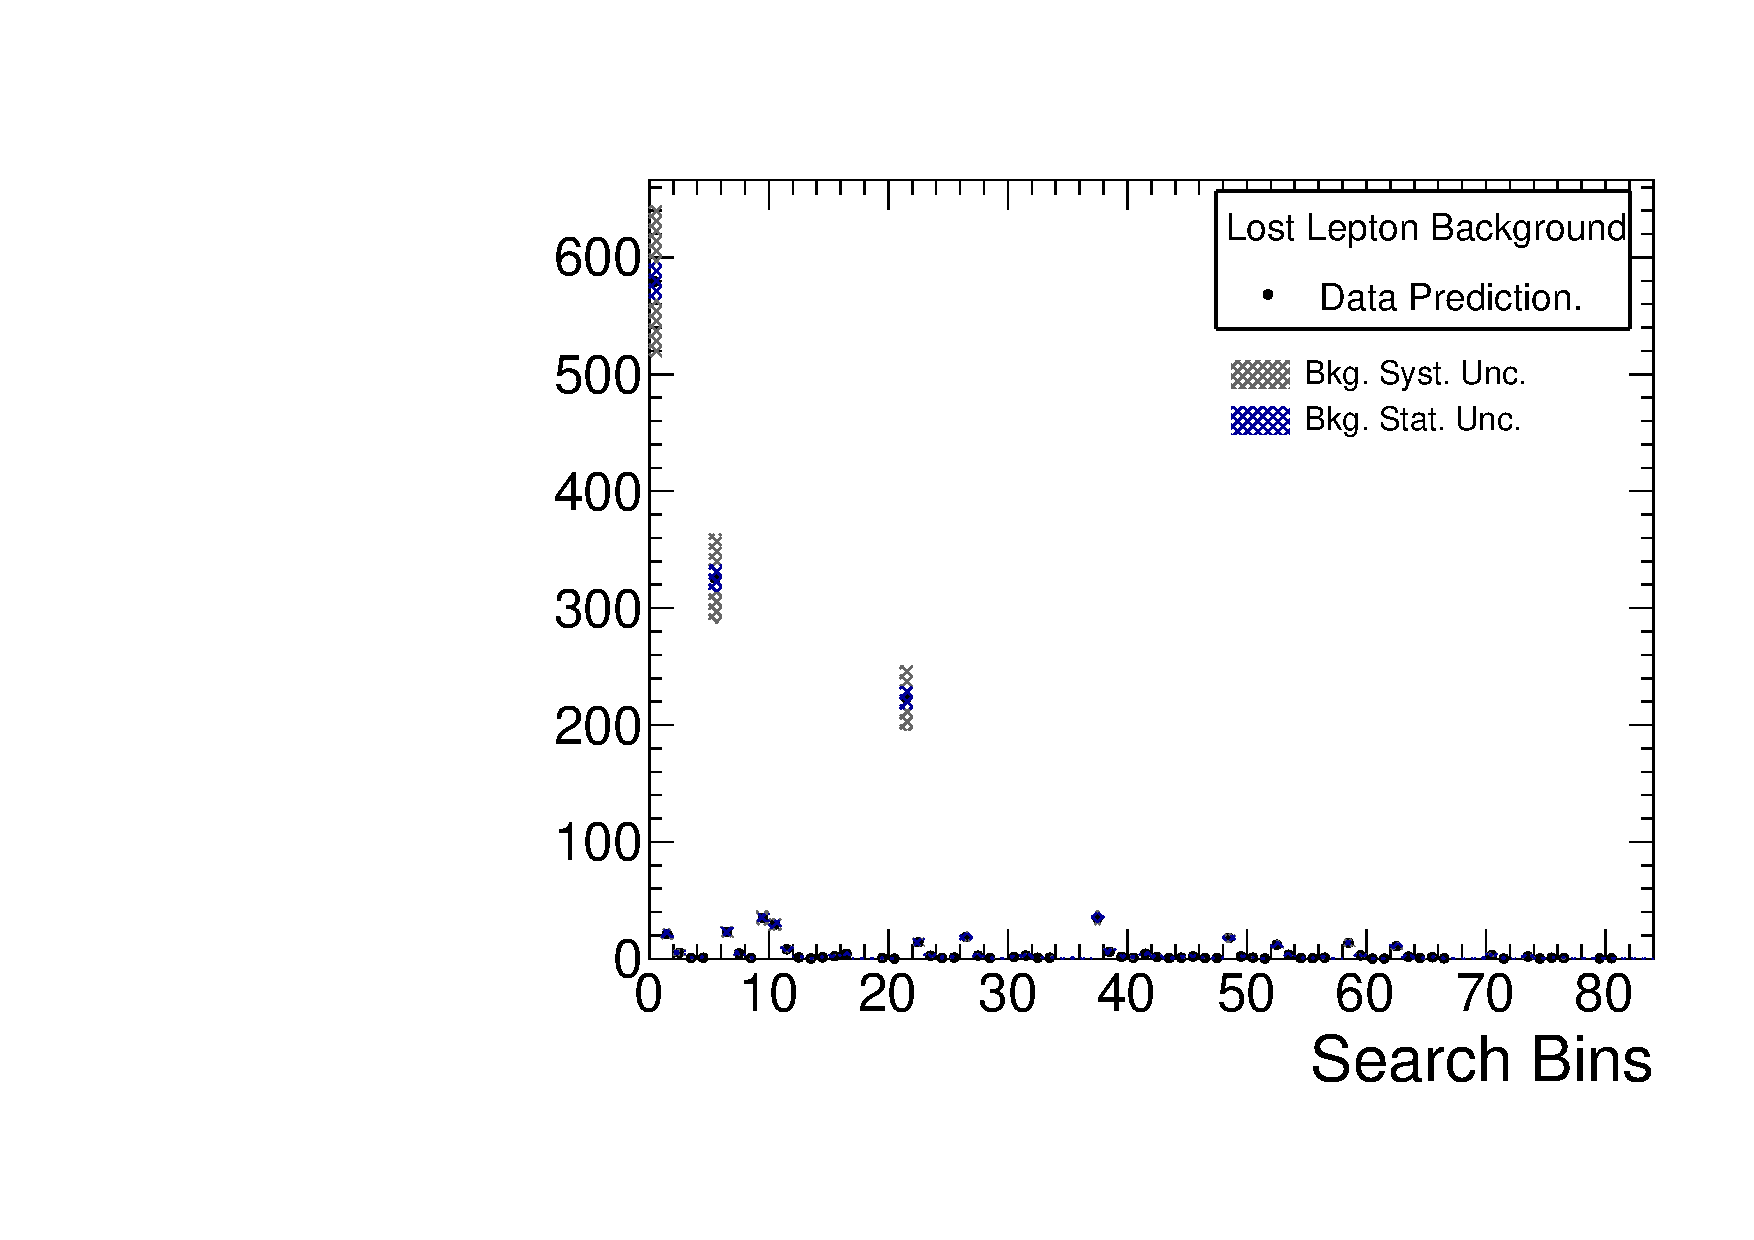
\includegraphics[angle=0,width=0.5\textwidth]{sections/mc4/Backgrounds/TF/figures/pred_full_lostle_comb.pdf}
  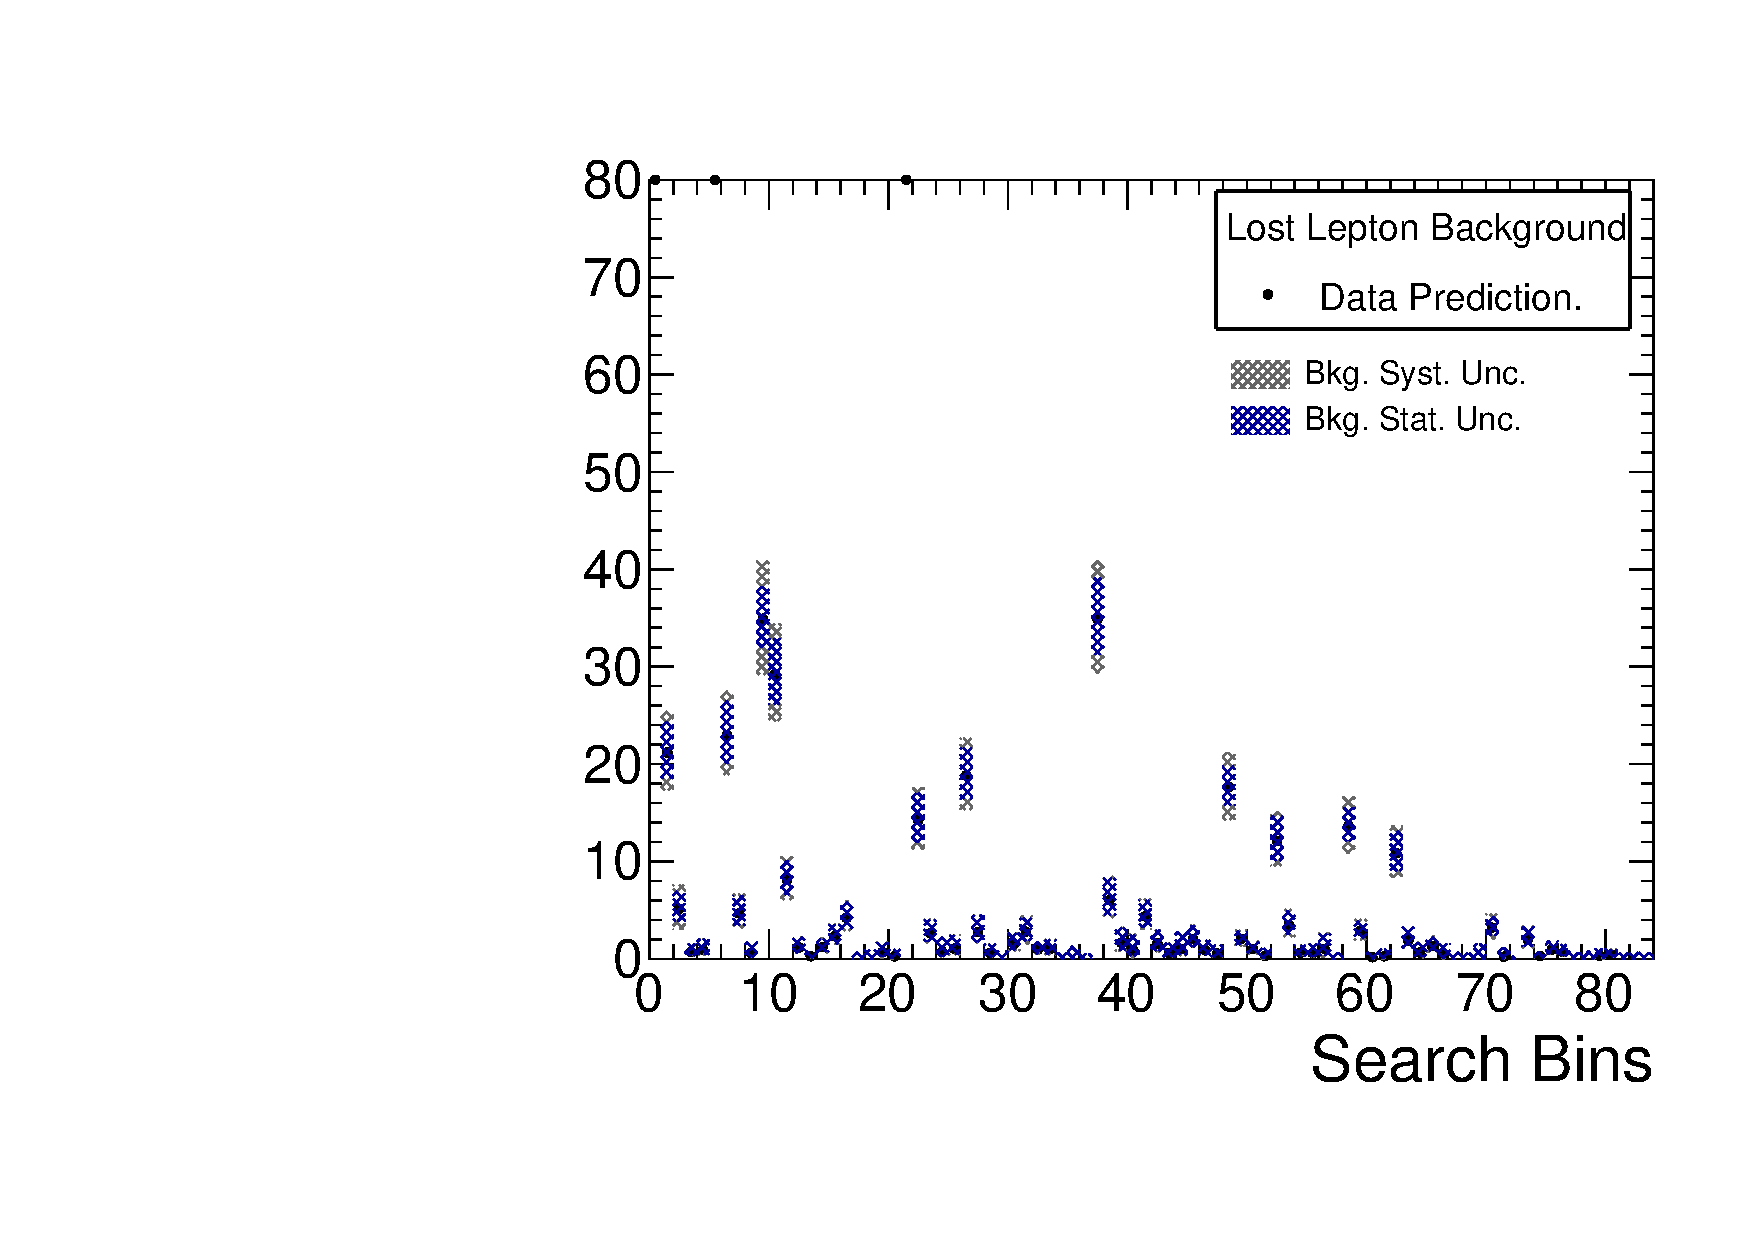
\includegraphics[angle=0,width=0.5\textwidth]{sections/mc4/Backgrounds/TF/figures/pred_zoomin_lostle_comb.pdf}
  \end{tabular}
  \caption{Predicted lost lepton background yield for a $35.9$~fb$^{-1}$ data for all the search regions. Right plot is a zoomed version of left plot.
Both statistical and total systematic uncertainties are shown. }
    \label{fig:LLpredictionSB}
  \end{center}
\end{figure}

